\section{\textsc{Принцип позиционирования GPS}}

Принцип позиционирования GPS довольно прост.
Рассмотрим приёмник, который измеряет до определённого спутника расстояние $R_1$, чьё месторасположение известно из эфемерид, передающихся в навигационном сообщении.
Приёмник знает, что он должен находиться где-то на поверхности сферы радиуса $R_1$.
Если добавить расстояние до второго спутника $R_2$, то приёмник будет знать, что он должен находиться не только на поверхности сферы радиуса $R_1$, но и на поверхности сферы радиуса $R_2$, т.е. на пересечении двух сфер (окружности).
Наконец, если добавить расстояние до третьего спутника $R_3$, то третья сфера будет пересекать первые две.
В итоге, все три сферы будут пересекаться только в двух точках, как показано на рис. \ref{fig-positioning}.
Одна из этих точек даёт бессмысленное решение навигационной задачи, например, она может находиться слишком далеко от поверхности Земли или двигаться с нереальной скоростью.
Следовательно, приёмник может просто отбросить эту точку, тем самым определить своё истинной месторасположение. 
\vspace{1em}
\begin{figure}[h]
\centering    
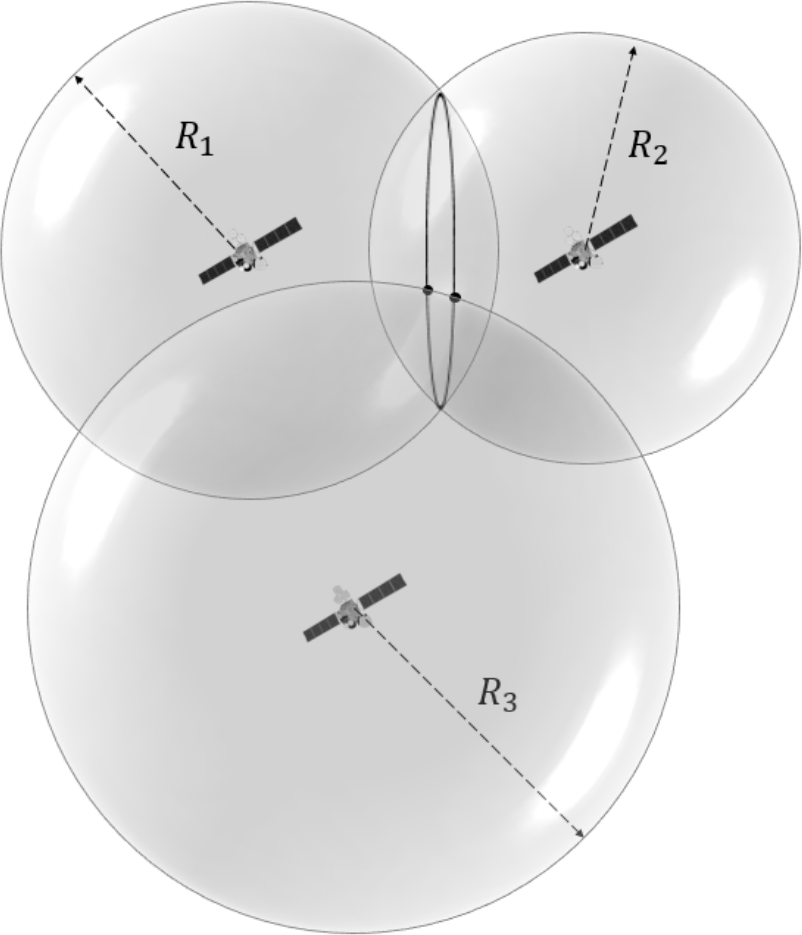
\includegraphics[width=0.3\linewidth]{fig/positioning.png}    
\caption{Визуализация GPS позиционирования.}
\label{fig-positioning}      
\end{figure}

В теории, для позиционирования необходимы только три спутника, как в примере приведённом выше.
Однако это относится только к безошибочным измерениям.
Большинство источников ошибок (см. ГЛАВА 1. Источники ошибок GPS) могут быть смоделированы и учтены, но ошибка часов приёмника вместо этого должна выступать четвертой неизвестной переменной.
Таким образом, на практике для позиционирования требуется дополнительный четвёртый спутник.

Приёмник GPS может вычислить своё расстояние до спутника при помощи нескольких типов измерений (см. ГЛАВА 1. Измерения GPS), а именно псевдодальности, фазы несущей и доплеровского сдвига.
В качестве примера рассмотрим технику позиционирования на основе измерений псевдодальности.

Подводя итог, схема процесса позиционирования состоит из следующих шагов:
\begin{enumerate}[wide,nosep]
\item Спутник генерирует несущую частоту и модулирует её кодом ранжирования (PRN кодом) и навигационным сообщением.
PRN код включает в себя информацию о времени передачи сигнала. 
\item Сгенерированный сигнал движется к поверхности Земли со скорость света в вакууме.
\item Приёмник получает сигнал и измеряет время его прихода.
\item Приёмник декодирует PRN код для получения времени передачи сигнала и навигационное сообщение для получения эфемерид (координат) спутника.
\item Используя всю эту информацию, приёмник рассчитывает псевдодальность до спутника.
\item Эта процедура выполняется по крайней мере для четырёх спутников одновременно, тем самым приёмник определяет своё месторасположения.
\end{enumerate}

Учитывая важные источники ошибок, можно исключить $e_r^s$ из выражения \eqref{eq-pr2}:
\begin{equation}
\prescript{*}{}R_r^s=\sqrt{(x_r-x^s)^2+(y_r-y^s)^2+(z_r-z^s)^2}+c\delta_r
\end{equation}
где 
$\prescript{*}{}R_r^s$ -- так называемая OMC (Observed Minus Computed) псевдодальность. 
При всех дальнейших выкладках будут подразумеваться именно OMC измерения, но знак звёздочки для простоты будет опущен.
В таком случае система уравнений выглядит следующим образом:
\begin{equation}
\label{eq-pr-system}
\begin{cases}
R_r^{(1)}=\sqrt{(x_r-x^{(1)})^2+(y_r-y^{(1)})^2+(z_r-z^{(1)})^2}+c\delta_r \\ 
R_r^{(2)}=\sqrt{(x_r-x^{(2)})^2+(y_r-y^{(2)})^2+(z_r-z^{(2)})^2}+c\delta_r \\
R_r^{(3)}=\sqrt{(x_r-x^{(3)})^2+(y_r-y^{(3)})^2+(z_r-z^{(3)})^2}+c\delta_r \\
R_r^{(4)}=\sqrt{(x_r-x^{(4)})^2+(y_r-y^{(4)})^2+(z_r-z^{(4)})^2}+c\delta_r
\end{cases}
\end{equation}
В текущей форме эта система уравнений является нелинейной и трудно разрешимой.
Для её линеаризации можно использовать разложение в ряд Тейлора, что позволит использовать матричные методы для поиска решения. 

Уравнение псевдодальности является функций четырёх переменных, поэтому разложение в ряд Тейлора должно выполняться для каждой переменной отдельно.
Также необходимо сделать первоначальную оценку ошибки часов и положения приёмника.
Элементы этого начального вектора $\vec{x}_0=\left[x_{r,0}\,y_{r,0}\,z_{r,0}\,\delta_{r,0}\right]^T$ будут служить точками, относительно которых выполняется разложение. 
Таким образом, разложение в ряд Тейлора уравнения псевдодальности определяется выражением:
\begin{equation}
\label{eq-pr-taylor}
\begin{aligned}
R_r^s=R_{r,0}^s&+\frac{\partial R_{r,0}^s}{\partial x_r}(x_r-x_{r,0})+\frac{\partial R_{r,0}^s}{\partial y_r}(y_r-y_{r,0}) \\
&+\frac{\partial R_{r,0}^s}{\partial z_r}(z_r-z_{r,0})+\frac{\partial R_{r,0}^s}{\partial \delta_r}(\delta_r-\delta_{r,0})    
\end{aligned}
\end{equation}  
где
$R_{r,0}^s=\sqrt{(x_{r,0}-x^s)^2+(y_{r,0}-y^s)^2+(z_{r,0}-z^s)^2}+c\delta_{r,0}$ -- начальное измерение псведодальности. 
Если теперь определить $\Delta R_r^s=R_r^s-R_{r,0}^s$, $\Delta x=x_r-x_{r,0}$, $\Delta y=y_r-y_{r,0}$, $\Delta z=z_r-z_{r,0}$ и $\Delta \delta_r=\delta_r-\delta_{r,0}$, то можно переписать систему уравнений \eqref{eq-pr-system} в матричном виде:
\begin{equation}
\label{eq-pr-system2}
\begin{bmatrix}
\Delta R_r^{(1)} \\ 
\Delta R_r^{(2)} \\ 
\Delta R_r^{(3)} \\
\Delta R_r^{(4)} 
\end{bmatrix} = \begin{bmatrix}
\dfrac{\partial R_{r,0}^{(1)}}{\partial x_r}&\dfrac{\partial R_{r,0}^{(1)}}{\partial y_r}&\dfrac{\partial R_{r,0}^{(1)}}{\partial z_r}&\dfrac{\partial R_{r,0}^{(1)}}{\partial \delta_r} \\[1em] 
\dfrac{\partial R_{r,0}^{(2)}}{\partial x_r}&\dfrac{\partial R_{r,0}^{(2)}}{\partial y_r}&\dfrac{\partial R_{r,0}^{(2)}}{\partial z_r}&\dfrac{\partial R_{r,0}^{(2)}}{\partial \delta_r} \\[1em]
\dfrac{\partial R_{r,0}^{(3)}}{\partial x_r}&\dfrac{\partial R_{r,0}^{(3)}}{\partial y_r}&\dfrac{\partial R_{r,0}^{(3)}}{\partial z_r}&\dfrac{\partial R_{r,0}^{(3)}}{\partial \delta_r} \\[1em]
\dfrac{\partial R_{r,0}^{(4)}}{\partial x_r}&\dfrac{\partial R_{r,0}^{(4)}}{\partial y_r}&\dfrac{\partial R_{r,0}^{(4)}}{\partial z_r}&\dfrac{\partial R_{r,0}^{(4)}}{\partial \delta_r} 
\end{bmatrix} \begin{bmatrix}
\Delta x \\ 
\Delta y \\ 
\Delta z \\
\Delta \delta_r   
\end{bmatrix}    
\end{equation}    
С учётом того, что
$\frac{\partial R_{r,0}^s}{\partial x_r}=\frac{x_{r,0}-x^s}{\rho_{r,0}^s}$,
$\frac{\partial R_{r,0}^s}{\partial y_r}=\frac{y_{r,0}-y^s}{\rho_{r,0}^s}$,    
$\frac{\partial R_{r,0}^s}{\partial z_r}=\frac{z_{r,0}-z^s}{\rho_{r,0}^s}$
и $\frac{\partial R_{r,0}^s}{\partial \delta_r}=c$,  
где $\rho_{r,0}^s=\sqrt{(x_{r,0}-x^s)^2+(y_{r,0}-y^s)^2+(z_{r,0}-z^s)^2}$, система уравнений \eqref{eq-pr-system2} имеет следующий вид:   
\begin{equation}
\begin{bmatrix}
\Delta R_r^{(1)} \\ 
\Delta R_r^{(2)} \\ 
\Delta R_r^{(3)} \\
\Delta R_r^{(4)} 
\end{bmatrix} = \begin{bmatrix}
\dfrac{x_{r,0}-x^{(1)}}{\rho_{r,0}^{(1)}}&\dfrac{y_{r,0}-y^{(1)}}{\rho_{r,0}^{(1)}}&\dfrac{z_{r,0}-z^{(1)}}{\rho_{r,0}^{(1)}}&c \\[1em] 
\dfrac{x_{r,0}-x^{(2)}}{\rho_{r,0}^{(2)}}&\dfrac{y_{r,0}-y^{(2)}}{\rho_{r,0}^{(2)}}&\dfrac{z_{r,0}-z^{(2)}}{\rho_{r,0}^{(2)}}&c \\[1em]
\dfrac{x_{r,0}-x^{(3)}}{\rho_{r,0}^{(3)}}&\dfrac{y_{r,0}-y^{(3)}}{\rho_{r,0}^{(3)}}&\dfrac{z_{r,0}-z^{(3)}}{\rho_{r,0}^{(3)}}&c \\[1em]
\dfrac{x_{r,0}-x^{(4)}}{\rho_{r,0}^{(4)}}&\dfrac{y_{r,0}-y^{(4)}}{\rho_{r,0}^{(4)}}&\dfrac{z_{r,0}-z^{(4)}}{\rho_{r,0}^{(4)}}&c 
\end{bmatrix} \begin{bmatrix}
\Delta x \\ 
\Delta y \\ 
\Delta z \\
\Delta \delta_r   
\end{bmatrix}    
\end{equation} 
Или в более краткой форме:
\begin{equation}
\label{eq-pr-system3}
\vec{y}_1=\textbf{A}\vec{x}_{\Delta,1}   
\end{equation} 
где
$\vec{y}_1$ -- известный вектор;
$\textbf{A}$ -- расчётная матрица;
$\vec{x}_{\Delta,1}$ -- неизвестный вектор.  
Следовательно, чтобы найти неизвестный вектор $\vec{x}_{\Delta,1}$ достаточно просто умножить левую часть уравнения \eqref{eq-pr-system3} на $\textbf{A}^{-1}$:
\begin{equation}
\vec{x}_{\Delta,1}=\textbf{A}^{-1}\vec{y}_1   
\end{equation}  
Следует обратить внимание, что обратная матрица $\textbf{A}^{-1}$ всегда существует, потому что уравнения пседодальности, соответствующие разным спутникам, линейно независимы.

Теперь для новой оценки ошибки часов и положения приёмника можно использовать:
\begin{equation}
\label{eq-solution}
\vec{x}_1=\vec{x}_0+\vec{x}_{\Delta,1}    
\end{equation}
Элементы вектора $\vec{x}_1$ также можно использовать в качестве точек разложения в ряде \eqref{eq-pr-taylor}.
Это, в свою очередь, приведёт к новым векторам $\vec{y}_2$ и $\vec{x}_{\Delta,2}$ и так далее.   
Таким образом, решение \eqref{eq-solution} можно можно обобщить в виде:
\begin{equation}
\vec{x}_n=\vec{x}_{n-1}+\vec{x}_{\Delta,n}    
\end{equation}
При каждом новом шаге элементы вектора $\vec{x}_{\Delta,n}$ уменьшаются (стремятся к нулю), поэтому итеративное решение можно продолжать вплоть до тех пор, пока $\vec{y}_n$ не станет равен $\vec{x}_n$. 
Это и будет соответствовать истинному месторасположению приёмника.

Строго говоря, элементы $\vec{x}_{\Delta,n}$ никогда не будут точно равны нулю, но алгоритм приёмника может быть установлен на прекращение, когда $|\vec{x}_{\Delta,n}|$ будет меньше определённого порогового значения, например, 1 см. 